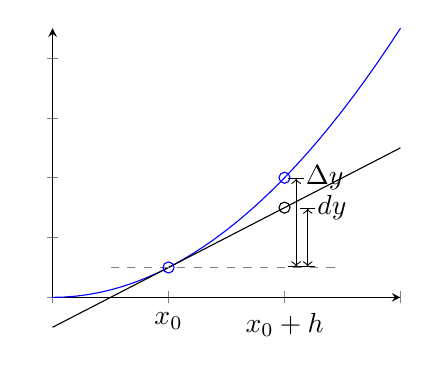
\begin{tikzpicture}
\begin{axis}[
    clip=false,
    width=6cm, height=5cm,
    axis lines=left,
    domain=0:2.5,samples=31,
    xmin=0, xmax=3,
    ymin=0, ymax=9,
    xticklabels={{},{},{$x_0$},{$x_0+h$},{}},
    yticklabels={},
]

    % Plots
    \addplot[domain=0:3,samples=31,blue,mark=none] {x^2};
    \addplot[blue,mark=o,only marks] coordinates {(1,1)(2,4)};
    \addplot[domain=0:3,samples=2,black,mark=none] {2*x-1};
    \addplot[black,mark=o,only marks] coordinates {(2,3)};

    % Labels
    \draw[dashed,gray] (axis cs:0.5,1) -- (axis cs:2.5,1);
    \draw[|<->|] (axis cs:2.2,1) -- (axis cs:2.2,3) node[anchor=west] {$dy$};
    \draw[|<->|] (axis cs:2.1,1) -- (axis cs:2.1,4) node[anchor=west] {$\Delta y$};

\end{axis}
\end{tikzpicture}